\documentclass[compress,red]{beamer}
\usepackage[utf8]{inputenc}
\usepackage{ucs}
\usepackage{amsmath}
\usepackage{amsfonts}
\usepackage{amssymb}
\usepackage[russian]{babel}
\usepackage{graphicx}
\usepackage{wrapfig}

\usepackage{tikz}
\usepackage{verbatim}

\usepackage{color}
\usepackage{xcolor}
\usepackage{listings}

\usepackage{caption}

\lstset{
language=ruby,
extendedchars=\true,
inputencoding=utf8x,
commentstyle=\itshape,
stringstyle=\bf,
belowcaptionskip=5pt }


\DeclareCaptionFont{white}{\color{white}}
\DeclareCaptionFormat{listing}{\colorbox{gray}{\parbox{\textwidth}{#1#2#3}}}
\captionsetup[lstlisting]{format=listing,labelfont=white,textfont=white}

\usetikzlibrary{calc,trees,positioning,arrows,chains,shapes.geometric,%
    decorations.pathreplacing,decorations.pathmorphing,shapes,%
    matrix,shapes.symbols}

\tikzset{
>=stealth',
  punktchain/.style={
    rectangle, 
    rounded corners, 
    % fill=black!10,
    draw=black, very thick,
    text width=10em, 
    minimum height=3em, 
    text centered, 
    on chain},
  line/.style={draw, thick, <-},
  element/.style={
    tape,
    top color=white,
    bottom color=blue!50!black!60!,
    minimum width=8em,
    draw=blue!40!black!90, very thick,
    text width=10em, 
    minimum height=1.5em, 
    text centered, 
    on chain},
  every join/.style={->, thick,shorten <=1pt},
  decoration={brace},
  tuborg/.style={decorate},
  tubnode/.style={midway, right=2pt},
}

\mode<presentation>

\usetheme{Warsaw}

\definecolor{Red}{rgb}{1,0,0}
\definecolor{Blue}{rgb}{0,0,1}
\definecolor{Green}{rgb}{0,1,0}
\definecolor{magenta}{rgb}{1,0,.6}
\definecolor{lightblue}{rgb}{0,.5,1}
\definecolor{lightpurple}{rgb}{.6,.4,1}
\definecolor{gold}{rgb}{.6,.5,0}
\definecolor{orange}{rgb}{1,0.4,0}
\definecolor{hotpink}{rgb}{1,0,0.5}
\definecolor{newcolor2}{rgb}{.5,.3,.5}
\definecolor{newcolor}{rgb}{0,.3,1}
\definecolor{newcolor3}{rgb}{1,0,.35}
\definecolor{darkgreen1}{rgb}{0, .35, 0}
\definecolor{darkgreen}{rgb}{0, .6, 0}
\definecolor{darkred}{rgb}{.75,0,0}

\xdefinecolor{olive}{cmyk}{0.64,0,0.95,0.4}
\xdefinecolor{purpleish}{cmyk}{0.75,0.75,0,0}

\useoutertheme[subsection=false]{smoothbars}

\title{Разбор итоговых задач}
\author{Информатика \\ 10-11 классы}

%\usecolortheme{dolphin}


\begin{document}
%%титульная страница
\maketitle
%% основные моменты

\section{Задача 1}

\subsection{Массивы}
\begin{frame}[fragile]
  \frametitle{Задача 1}
  \begin{itemize}
    \item Дан целочисленный массив из 30 элементов. Элементы могут принимать значения от 0 до 100 – баллы, полученные на ЕГЭ. Опишите на русском языке или на одном из языков программирования алгоритм, который подсчитывает и выводит средний балл учащихся, сдавших экзамен (получивших оценку более 20 баллов). Гарантируется, что хотя бы один ученик в классе успешно сдал экзамен.
  \end{itemize}
\end{frame}

\subsection{Пример}
\begin{frame}[fragile]
  \frametitle{Пример}
  \centerline{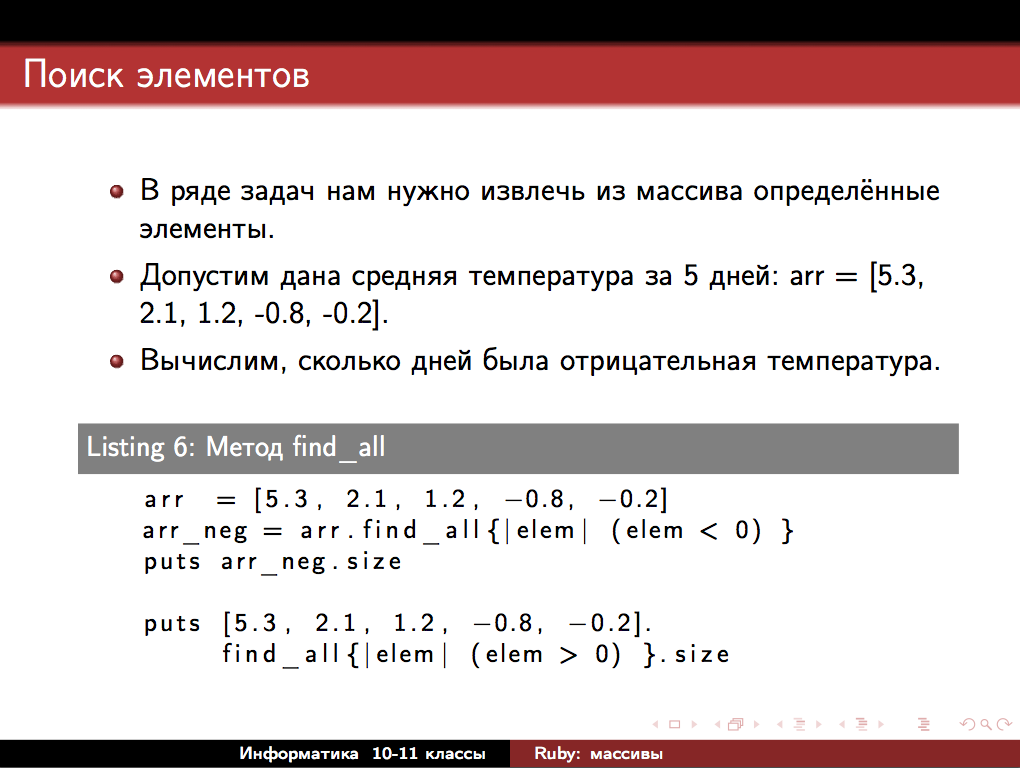
\includegraphics[width=0.8\textwidth]{images/screen1.png}}
  \centerline{Презентация №4 --- массивы}
\end{frame}

\subsection{Пример 2}
\begin{frame}[fragile]
  \frametitle{Пример}
  \centerline{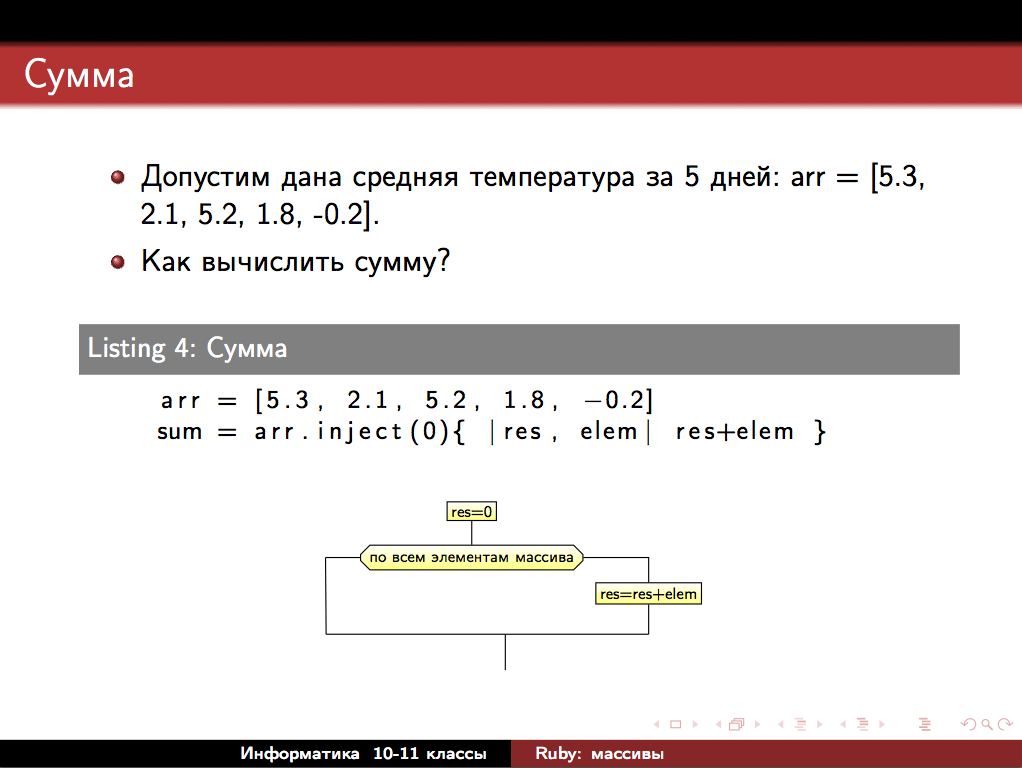
\includegraphics[width=0.8\textwidth]{images/screen2.png}}
  \centerline{Презентация №4 --- массивы}
\end{frame}

\subsection{Решение}
\begin{frame}[fragile]
  \frametitle{Решение задачи 1}
  \scriptsize{
  \begin{lstlisting}[language=ruby,basicstyle=\footnotesize,label=ruby1,caption=Решение задачи 1]
    arr = [20, 87, 23, 53, 100, 2]
    passed = arr.find_all{ |elem| elem > 20 }
    sum_passed = passed.inject(0){ |res, elem| res+elem }
    average = sum_passed / passed.size
    puts average
  \end{lstlisting}
  }
  \begin{itemize}
    \item Задаём исходные данные.
    \item Находим тех, кто сдал + сумму их баллов.
    \item Делим сумму на количество и выводим результат.
  \end{itemize}
\end{frame}

\section{Задача 4}
\subsection{Четыре}
\begin{frame}[fragile]
  \frametitle{Диофантовы уравнения}
  \begin{itemize}
    \item Напишите эффективную программу, находящую все решения линейного диофантова уравнения $ax+by=c$,
    \item где $a, b, c$ --- натуральные числа, задающиеся в начале программы, $x, y$ --- неизвестные (\textbf{целые числа}).
    \item Ограничение: $|x|,|y| < 100$; то есть надо найти решения, где оба неизвестных не превосходят $100$.
  \end{itemize}
\end{frame}

\subsection{Метод перебора}
\begin{frame}[fragile]
  \frametitle{Метод перебора}
  \centerline{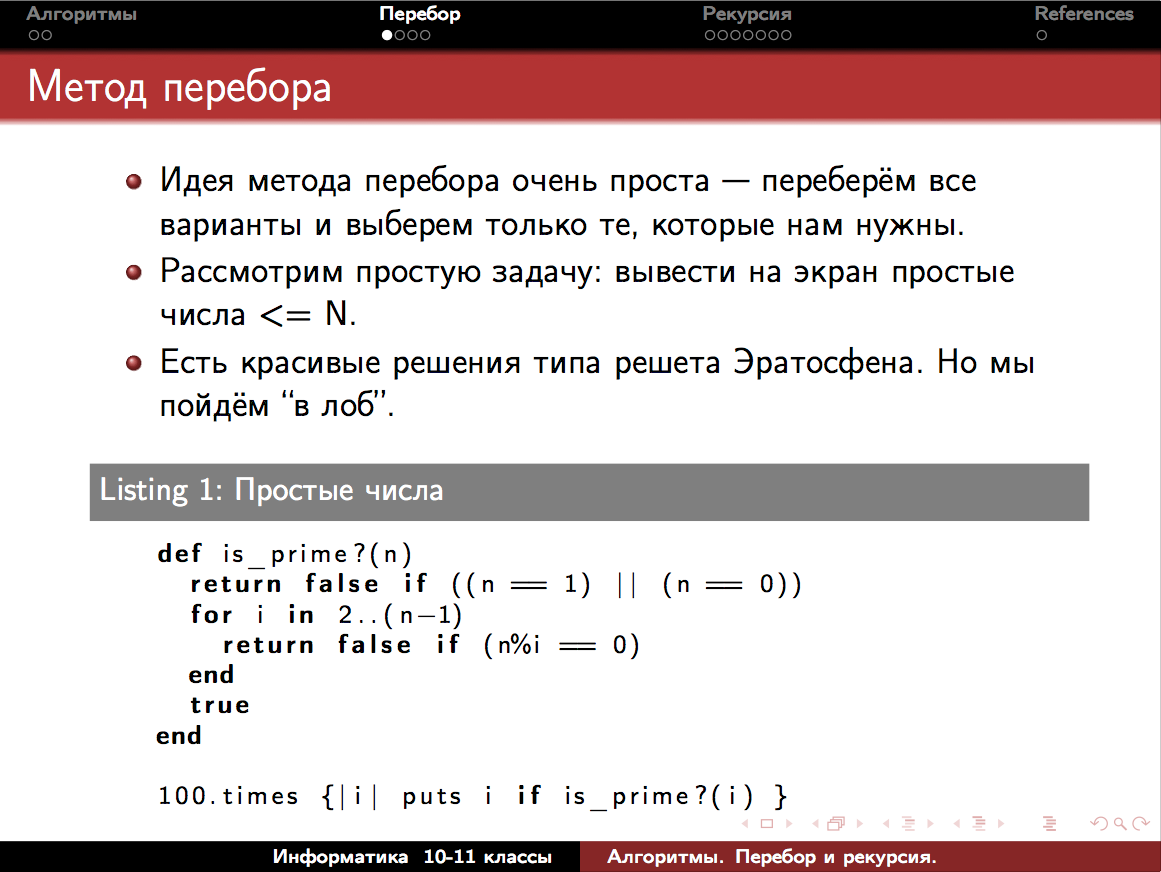
\includegraphics[width=0.8\textwidth]{images/screen3.png}}
  \centerline{Презентация №9 --- перебор и рекурсия}
\end{frame}

\subsection{Алгоритм решения задачи 4}
\begin{frame}[fragile]
  \frametitle{Алгоритм решения задачи 4}
  \begin{enumerate}
    \item Переберём все возможные пары $(x,y)$ от -100 до 100.
    \item Подставим каждую из них в уравнение $ax+by=c$.
    \item Если полученное равенство будет истинным, выведем на экран значения $(x,y)$.
  \end{enumerate}
\end{frame}

\subsection{Решение задачи 4}
\begin{frame}[fragile]
  \frametitle{Решение задачи 4}
  \scriptsize{
  \begin{lstlisting}[language=ruby,basicstyle=\footnotesize,label=ruby2,caption=Задача 4]
  a = 12
  b = 16
  c = 100
  for x in -100..100
    for y in -100..100
      puts "x = #{x}, y = #{y}" if (a*x + b*y == c)
    end
  end
  \end{lstlisting}
  }
  
\end{frame}

\section{Задача 2}
\subsection{Задача 2}
\begin{frame}[fragile]
  \frametitle{Задача 2}
  \begin{itemize}
    \item Напишите программу, подсчитывающую максимальное количество подряд идущих отрицательных элементов в целочисленном массиве длины 30.
    \item \textbf{Решение}.
    \item 1, -2, -5, 9, 1, -4, 3, 0, -5, -1, -3, -4, 0, -1
    \item Ответ: 4. Давайте посмотрим, как мы в уме находим это количество?
    \item Мы просматриваем все числа слева направо. Ищем первое отрицательное.
    \item Далее, считаем количество отрицательных чисел, идущих после первого.
    \item Дойдя до положительного числа, запоминаем, сколько пока было максимально подряд идущих элементов.
  \end{itemize}
\end{frame}

\subsection{Разбор задачи 2}
\begin{frame}[fragile]
  \frametitle{Задача 2. Решение.}
  \begin{itemize}
    \item 1, -2, -5, 9, 1, -4, 3, 0, -5, -1, -3, -4, 0, -1
    \item На примере: идём до числа -2.
    \item Считаем количество идущих за ним отрицательных элементов. Их будет 2. Запоминаем это число.
    \item Пропускаем 9 и 1, так как они --- положительные.
    \item Берём -4. Считаем количество идущих после -4 отрицательных чисел. Их нет. Значит, в данной группе всего 1 число. Ранее было 2. 
    \item Значит, максимальное число подряд идущих отрицательных элементов так и остаётся равным 2.
    \item Идём далее. 0 пропускаем, доходим до -5. Там --- 4 подряд идущих отрицательных элемента.
    \item $4>2$, поэтому запоминаем число 4, как текущий максимум. Продолжаем так до конца.
  \end{itemize}
\end{frame}

\subsection{Разбор задачи 2 - 2}
\begin{frame}[fragile]
  \frametitle{Формализация}
  \begin{itemize}
    \item Итого, что нам надо две переменных:
      \begin{enumerate}
        \item Переменная, в которой мы будем хранить текущее найденное максимальное количество подряд идущих элементов массива (max).
        \item Переменная, в которой мы будем хранить количество подряд идущих отрицательных элементов в одной группе (current).
      \end{enumerate}
  \end{itemize}
  
  
  \begin{tabular}{|c|c|c|c|c|c|c|c|c|c|c|c|c|c|c|c|c|c|}
    \hline
    Число   & 1 & -2 & -5 & 9 & 1 & -4 & 3 & 0 & -5 & -1 & -3 & -4 & 0 & -1 \\ \hline
    current & 0 & 1 & 2 & 0 & 0 & 1 & 0 & 0 & 1 & 2 & 3 & 4 & 0 & 1 \\ \hline
    max     & 0 & 1 & 2 & 2 & 2 & 2 & 2 & 2 & 2 & 2 & 3 & 4 & 4 & 4 \\ \hline
  \end{tabular}
  
\end{frame}

\subsection{Условия}
\begin{frame}[fragile]
  \frametitle{Формализация условий}
  \begin{itemize}
    \item Формализуем условия, при которых изменяются переменные \emph{current} и \emph{max}.
    \item Если пробегаемое число --- отрицательное, то увеличиваем current на единицу:
    \item current += 1 if elem < 0.
    \item Если пробегаемое число больше или равно нулю, то обнуляем current:
    \item current = 0 if elem >= 0.
    \item Если количество элементов в группе превысило максимальное, изменяем последнее:
    \item max = current if current > max.
  \end{itemize}
\end{frame}

\subsection{Программа для задачи 2}
\begin{frame}[fragile]
  \frametitle{Программа для задачи 2}
  
  \scriptsize{
  \begin{lstlisting}[language=ruby,basicstyle=\footnotesize,label=ruby3,caption=Задача 2]
    arr = [1, -2, -5, 9, 1, -4, 3, 0, -5, -1, -3, -4, 0, -1]
    current = 0
    max = 0
    for i in 0..arr.size-1
      current += 1 if arr[i] < 0
      current = 0  if arr[i] >= 0
      max = current if current > max
    end
    puts max
  \end{lstlisting}
  }
  
\end{frame}

\subsection{Альтернатива для задачи 2}
\begin{frame}[fragile]
  \frametitle{Альтернативное решение}
  \scriptsize{
  \begin{lstlisting}[language=ruby,basicstyle=\footnotesize,label=ruby4,caption=Альтернативное решение задачи 2]
    arr = [1, -2, -5, 9, 1, -4, 3, 0, -5, -1, -3, -4, 0, -1]
    current = 0
    max = 0
    arr.each do |elem|
      current += 1 if elem < 0
      current = 0  if elem >= 0
      max = current if current > max
    end
    puts max
  \end{lstlisting}
  }
  
\end{frame}

\section{References}
\subsection{References}
\begin{frame}[fragile]
  \frametitle{References}
  \begin{itemize}
    \item При подготовке данного материала использовались сайты: http://ru.wikibooks.org/wiki/Ruby, http://rubydev.ru, http://en.wikipedia.org, http://ruby-lang.org.
    \item Все презентации доступны на http://school.smirik.ru!
    \item Вопросы, предложения, д/з: smirik@gmail.com
  \end{itemize}
\end{frame}

\end{document}